To validate this methodology, finite element simulations were performed using the Maxwell3D package from ANSYS Electronics Desktop 2018.0 (ANSYS, Inc., Berkeley, CA, USA). Two cases were considered, with the magnetic field of each being calculated analytically using the above methodology and numerically using Maxwell3D. The second case was further validated using the analytic solutions presented by \textcite{Caciagli2018}. The magnetic field for both cases was also calculated using methodology from previously published and validated work by the current authors \cite{OConnell2020}. In the subsequent sections, the results and computation time from the current methodology are compared to those of the finite element simulations, literature, and earlier work.

\subsection{Pyramid frustum magnet}

\begin{figure}
	\centering
	\def\lim{13}

\tdplotsetmaincoords{70}{45}
\begin{tikzpicture}[scale=0.13,tdplot_main_coords]

% Define coordinates:
\coordinate(ppb) at (15,15,-20);
\coordinate(pnb) at (15,-15,-20);
\coordinate(nnb) at (-15,-15,-20);
\coordinate(npb) at (-15,15,-20);
\coordinate(ppt) at (10,10,0);
\coordinate(pnt) at (10,-10,0);
\coordinate(nnt) at (-10,-10,0);
\coordinate(npt) at (-10,10,0);

% Fill in polygons:
\filldraw[fill=white] (ppt) -- (pnt) -- (nnt) -- (npt) -- cycle;
\filldraw[fill=white] (ppt) -- (ppb) -- (pnb) -- (pnt) -- cycle;
\filldraw[fill=white] (pnt) -- (nnt) -- (nnb) -- (pnb) -- cycle;

% Axes:
\draw[->] (0,0,0) -- (\lim,0,0);
\draw[->] (0,0,0) -- (0,\lim,0);
\draw[->] (0,0,0) -- (0,0,\lim);
\node(xaxis) at (\lim+2,0,0) {\(x\)};
\node(yaxis) at (0,\lim+2,0) {\(y\)};
\node(zaxis) at (0,0,\lim+2) {\(z\)};

% Dimensions:
\draw[<->] (20,-18,-20) -- (20,12,-20);
\node(botdim) at (26,-5,-20) {30mm};
\draw[<->] (-12,-20,-20) -- (18,-20,-20);
\node(botdim2) at (5,-26,-20) {30mm};
\draw[<->] (-15,-7,0) -- (-15,13,0);
\node(topdim) at (-21,6,0) {20mm};
\draw[<->] (-6,-15,0) -- (14,-15,0);
\node(topdim2) at (6,-21,0) {20mm};
\draw[<->] (17,17,-20) -- (17,17,0);
\node(height) at (21,21,-10) {20mm};

\end{tikzpicture}
	\caption{A square pyramid frustum permanent magnet. It has a base length of 30\si{\milli\metre}, a top length of 20\si{\milli\metre}, a height of 20\si{\milli\metre}, and a magnetisation of \num{1.035e6}\si{\ampere\per\metre} (1.3\si{\tesla}) in the positive \(z\) direction.}
	\label{fig:p2frustum}
\end{figure}

To validate Equation (\ref{eqn:p2fieldequation}) for non-cuboid magnets, the magnetic field due to the pyramid frustum permanent magnet shown in Figure \ref{fig:p2frustum} was computed. This frustum has a base length of 30\si{\milli\metre}, a top length of 20\si{\milli\metre}, a height of 20\si{\milli\metre}, and a magnetisation of \num{1.035e6}\si{\ampere\per\metre} (1.3\si{\tesla}) in the \(z\)-direction; i.e., a magnetisation vector of \(\left[0,0,1.035 \times 10^6\right]\)\si{\ampere\per\metre}. The magnetic field is measured across a plane positioned 1mm above the top surface of the frustum using a \(301\times301\) grid of points on a 30\si{\milli\metre} \(\times\) 30\si{\milli\metre} region (0.1\si{\milli\metre} grid spacing using 90601 gridpoints).

The geometry was input into both Maxwell3D and Matlab code, with the Maxwell3D simulation using approximately \num{1.2e6} tetrahedral elements (approx. \num{2e5} inside the magnet and \num{1e6} in the region outside the magnet). Both the Matlab code and Maxwell3D simulations were used to calculate the field across the previously mentioned \(301\times301\) grid of points above the frustum magnet, with results shown in Figure \ref{fig:p2frustumfield}.

The maximum field strength was 0.633\si{\tesla} (this work) and 0.636\si{\tesla} (FEA), giving a difference of 0.5 percent. Over the entire grid of points, the maximum error was 0.7 percent. This indicates that the analytic work presented in this paper is giving accurate field results. More detailed results are given in \ref{sec:p2detailedResults}.

The analytic work presented here and the FEA simulations calculate the magnetic field in very different ways, and as such it is difficult to compare the computation time for each method. For the frustum above, the FEA simulation took approximately 40 minutes, but the field can be found at any number of points after the simulation has been completed. In contrast, the analytic work presented here requires more computational time as the number of field points is increased. However, even with a relatively large number of field calculations, this algorithm took approximately 0.3 seconds to calculate the field at all 90601 points.

Finally, this calculation was validated using previous published and validated work by the current authors \cite{OConnell2020}. The error was within numerical noise, but the work presented in this paper was able to calculate the field orders of magnitude faster.

\begin{figure}
	\centering
	\begin{subfigure}{0.65\textwidth}
		\centering
		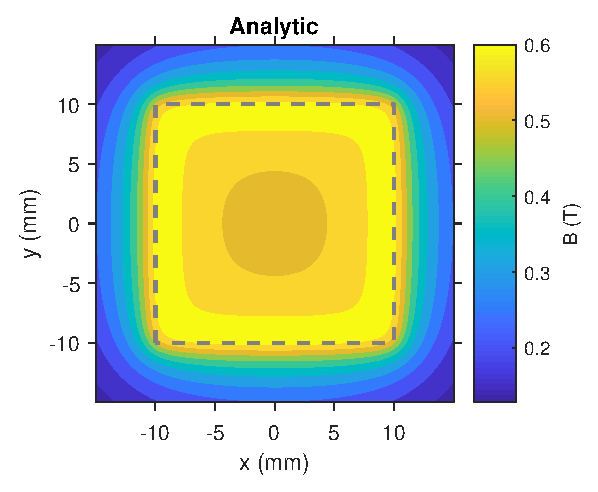
\includegraphics[width=\textwidth]{p2/p2FIG5a}
		\caption{}\label{fig:frustumfielda}\vspace{5mm}
	\end{subfigure}
	
	\begin{subfigure}{0.65\textwidth}
		\centering
		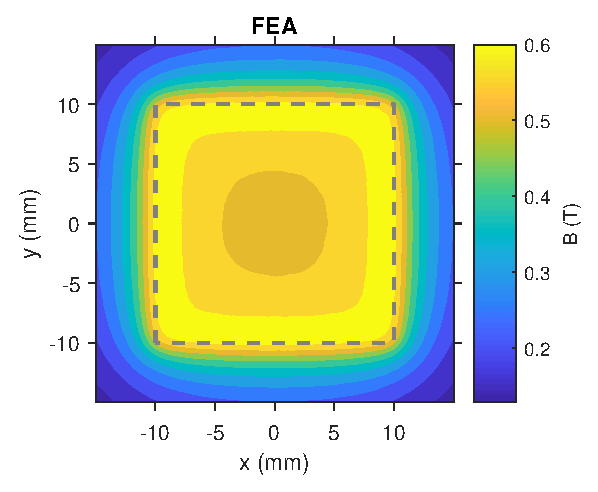
\includegraphics[width=\textwidth]{p2/p2FIG5b}
		\caption{}\label{fig:frustumfieldb}
	\end{subfigure}
	\caption{Magnetic field strength 1mm above the pyramid frustum magnet shown in Figure \ref{fig:p2frustum}, with the top surface of the magnet shown as a dashed line. The analytic calculation is shown in (\subref{fig:frustumfielda}), with the finite element calculation in (\subref{fig:frustumfieldb}). The maximum error between the two calculations is 0.7 percent, showing strong agreement.}
	\label{fig:p2frustumfield}
\end{figure}

\subsection{Cylindrical magnet}\label{sec:p2cylindricalmagnet}
\begin{figure}
	\centering
	\def\lim{13}

\tdplotsetmaincoords{70}{0}
\begin{tikzpicture}[scale=0.14,tdplot_main_coords]

% Draw cylinder
\draw (-10,0,-20) arc[radius = 10, start angle = -180, end angle = 0];
\draw (0,0,0) circle [radius = 10];
\draw (-10,0,0) -- (-10,0,-20);
\draw (10,0,0) -- (10,0,-20);

% Axes:
\draw[->] (0,0,0) -- (\lim,0,0);
\draw[->] (0,0,0) -- (0,0,\lim);
\node(xaxis) at (\lim+2,0,0) {\(x\)};
\node(zaxis) at (0,0,\lim+2) {\(z\)};

% Dimensions:
\draw[<->] (0,0,-27) -- (10,0,-27);
\node(radius) at (5,0,-30) {10mm};
\draw[<->] (-15,0,-20) -- (-15,0,0);
\node(height) at (-20,0,-10) {20mm};

\end{tikzpicture}
	\caption{A cylindrical permanent magnet. It has a radius of 10\si{\milli\metre}, a height of 20\si{\milli\metre}, and a magnetisation of \num{1.035e6}\si{\ampere\per\metre} (1.3\si{\tesla}) in the positive \(z\) direction.}
	\label{fig:p2cylinder}
\end{figure}
To further validate the analytic algorithm, a cylindrical geometry was examined, as shown in Figure \ref{fig:p2cylinder}. This magnet is an axially-magnetised cylindrical magnet with a radius of 10\si{\milli\metre}, a height of 20\si{\milli\metre}, and a magnetisation strength of \num{1.035e6}\si{\ampere\per\metre} (1.3\si{\tesla}). The magnetic field is again measured across a plane positioned \(z = 1\)\si{\milli\metre} above the top surface of the magnet using a \(301\times301\) grid of points on a 30\si{\milli\metre} \(\times\) 30\si{\milli\metre} region (0.1\si{\milli\metre} grid spacing using 90601 gridpoints).

Firstly, the exact magnetic field was calculated using the analytic equations published by \textcite{Caciagli2018}. Then, the geometry was input into Maxwell3D and a simulation carried out using approximately \num{9.6e5} tetrahedral elements (approximately \num{1.7e5} inside the magnet and \num{7.9e5} in the region outside the magnet). The cylinder was finally approximated as a polygonal prism, with the cross section being a 32-gon and an equivalent radius to maintain the same volume as the cylinder. Equation (\ref{eqn:p2fieldequation}) was applied to this polygonal prism to approximate the solution of a cylindrical magnet using a polyhedral magnet, and the results of all three calculations shown in Figure \ref{fig:p2cylinderfield}.

The maximum field strength was 0.571\si{\tesla} (this work), 0.573\si{\tesla} (FEA), and 0.571\si{\tesla} (exact \cite{Caciagli2018}). When compared to the exact result, the polyhedral approximation using this work gives a maximum error of less than 0.1 percent. When compared to the FEA simulation, the polyhedral approximation gave a maximum error of 0.8 percent. This implies the polyhedron is able to accurately approximate a cylindrical permanent magnet. More detailed results are given in \ref{sec:p2detailedResults}.

Again, it is difficult to compare the computation time of the algorithm presented in this paper and FEA simulations. The simulations took approximately 38 minutes to calculate the field at any number of points, whereas the algorithm here took approximately 0.9 seconds to calculate the field at 90601 points.

Additionally, this calculation was validated using previous published and validated work by the current authors \cite{OConnell2020}. The error was within numerical noise, but the algorithm presented in this paper calculated the field orders of magnitude faster.
\begin{figure}
	% Colour should be used for this figure
	\centering
	\begin{subfigure}{0.47\textwidth}
		\centering
		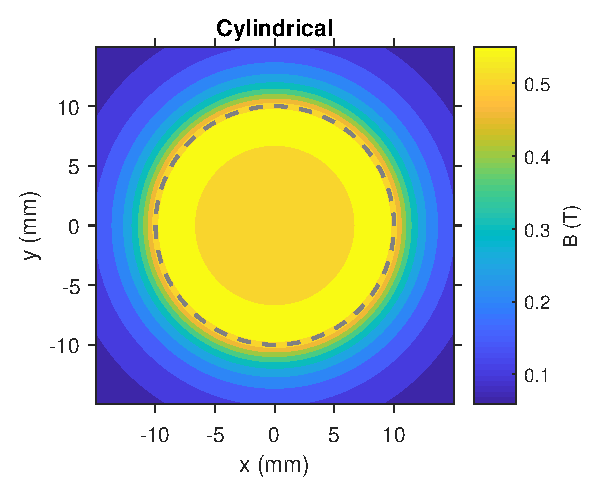
\includegraphics[width=\textwidth]{p2/p2FIG7a}
		\caption{}\label{fig:p2cylinderfielda}
	\end{subfigure}
	~
	\begin{subfigure}{0.47\textwidth}
		\centering
		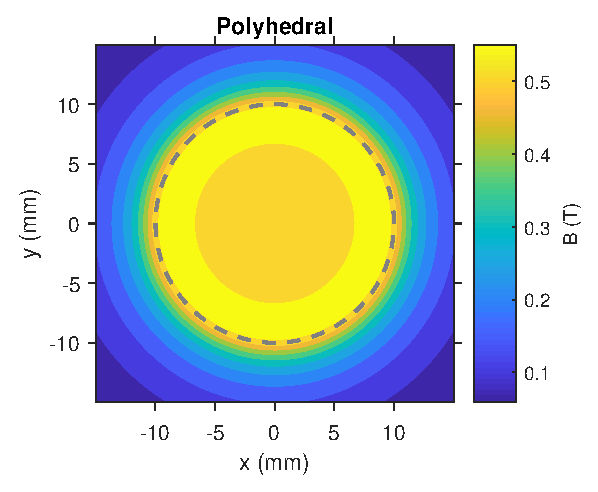
\includegraphics[width=\textwidth]{p2/p2FIG7b}
		\caption{}\label{fig:p2cylinderfieldb}
	\end{subfigure}
	
	\vfill
	\begin{subfigure}{0.47\textwidth}
		\centering
		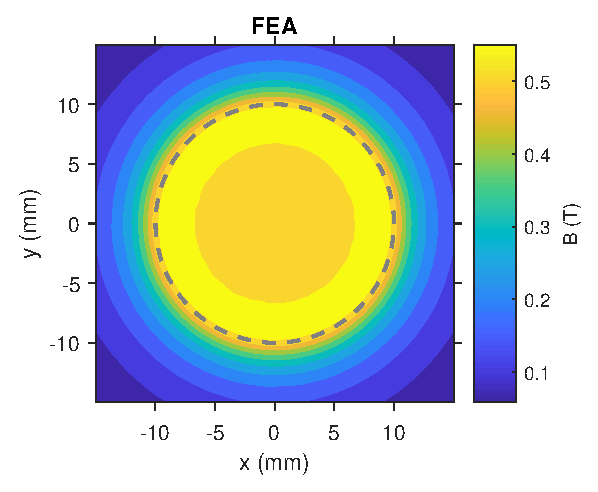
\includegraphics[width=\textwidth]{p2/p2FIG7c}
		\caption{}\label{fig:p2cylinderfieldc}
	\end{subfigure}
	\caption{Magnetic field strength 1\si{\milli\metre} above the cylindrical magnet shown in Figure \ref{fig:p2cylinder}, with the top surface of the magnet shown as a dashed line. The analytic cylindrical field \cite{Caciagli2018} is shown in (\subref{fig:p2cylinderfielda}), the polyhedral field shown in (\subref{fig:p2cylinderfieldb}), and the finite element calculation in (\subref{fig:p2cylinderfieldc}). The maximum percentage error between the exact cylinder field \cite{Caciagli2018} and polyhedral field was less than 0.1 percent, indicating it is an accurate approximation to a cylindrical magnet.}
	\label{fig:p2cylinderfield}
\end{figure}

\subsection{Polyhedral approximation of curved surfaces}
In the previous section, it was shown that an extruded 32-gon magnet is able to accurately approximate an axially-magnetised cylindrical magnet. This was validated using slow FEA simulations and the much faster analytic solution published by \textcite{Caciagli2018}. However, no analytic field solutions for general curved surfaces exist in literature, and FEA is slow and is impractical for real-time simulations. Instead, polyhedra can be used to approximate these surfaces for a fast-solving and accurate solution. To produce more accurate results, a polyhedron with a larger number of faces can be used; to achieve a faster calculation, a polyhedron with fewer faces can be used. This section shows an example of this tradeoff between accuracy and calculation time by approximating a cylindrical magnet with an extruded polygon with a varying number of sides, \(n\).

To quantify the error of the polyhedral approximation, the cylindrical magnet defined in Section \ref{sec:p2cylindricalmagnet} was considered. The magnetic field produced by this magnet was calculated using the equations published by \textcite{Caciagli2018} at a point 1\si{\milli\metre} above the central axis of the magnet, \(\mathbf{x} = \left[ 0, 0, 1\right]\)\si{\milli\metre}, and a point 1\si{\milli\metre} above the circumference of the top surface, \(\mathbf{x} = \left[ 10, 0, 1 \right]\)\si{\milli\metre}. The magnet was then approximated as a regular polygonal prism with a given number of sides \(n\), and the magnetic field calculated at the two aforementioned points. As the number of sides of the polygon \(n\) was increased, the error between the fields produced by cylindrical magnet and polyhedral magnet was calculated and recorded.

At the point \(\mathbf{x} = \left[ 0,0,1\right]\)\si{\milli\metre}, the exact magnetic field strength \cite{Caciagli2018} is 0.52\si{\tesla}. For a point along the axis of this magnet, the field can also be found using the difference between two cosines, giving the same result. The percentage error between this value and the magnetic field strength due to a polyhedral approximation was calculated for each \(n\) and is shown in Figure \ref{fig:p2polycylapproxa}. The polyhedral approximation is most impactful near the curved surface of the magnet, since this is where the geometry has been changed most significantly. Therefore, at the point \(\mathbf{x} = \left[ 0,0,1\right]\)\si{\milli\metre}, the polyhedral approximation is negligible and the error small since this point is far from the curved surface. The \(n = 32\) approximation from Section \ref{sec:p2cylindricalmagnet} takes approximately 28\si{\milli\second} to calculate the field and gives an error of \num{2.4e-5} percent. Alternatively, halving the number of sides (\(n = 16\)) takes approximately 17\si{\milli\second} to calculate the field while giving a larger error of \num{4.1e-4} percent.

At the point \(\mathbf{x} = \left[ 10,0,1\right]\)\si{\milli\metre}, the exact magnetic field strength \cite{Caciagli2018} is 0.53\si{\tesla}. The error between this field strength and the field strength due to the polyhedral approximation was again calculated and is shown in Figure \ref{fig:p2polycylapproxb}. This point is significantly closer to the curved surface of the magnet, and the error is therefore larger than at the point \(\left[ 0,0,1\right]\)\si{\milli\metre}. However, the error is still negligible for sufficiently large \(n\). The \(n = 32\) approximation from Section \ref{sec:p2cylindricalmagnet} takes approximately 29\si{\milli\second} to calculate the field and gives an error of \num{2.8e-2} percent. Alternatively, halving the number of sides (\(n = 16\)) takes approximately 16\si{\milli\second} to calculate the field while giving a larger error of \num{4.5e-1} percent.
\begin{figure}
	\centering
	\begin{subfigure}{0.6\textwidth}
		\centering
		\includegraphics[width=\textwidth]{p2/p2FIG8a}
		\caption{}\label{fig:p2polycylapproxa}
	\end{subfigure}
	
	\begin{subfigure}{0.6\textwidth}
		\centering
		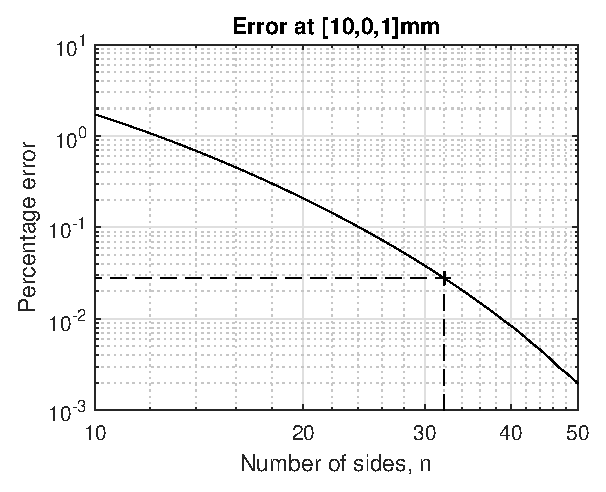
\includegraphics[width=\textwidth]{p2/p2FIG8b}
		\caption{}\label{fig:p2polycylapproxb}
	\end{subfigure}
	\caption{Error in the magnetic field strength produced by a polygonal prismatic magnet approximation of a cylindrical magnet as the number of sides of the polygon, \(n\), is increased. The \(n = 32\) approximation from Section \ref{sec:p2cylindricalmagnet} is highlighted. At the point \(\mathbf{x} = \left[0,0,1\right]\)\si{\milli\metre} (\subref{fig:p2polycylapproxa}), the magnetic field strength is 0.52\si{\tesla}, leading to an error of \num{2.4e-5} percent for a 32-gon approximation. At the point \(\mathbf{x} = \left[10,0,1\right]\)\si{\milli\metre} (\subref{fig:p2polycylapproxb}), the magnetic field strength is 0.53\si{\tesla}, leading to an error of \num{2.8e-2} percent for a 32-gon approximation.}
	\label{fig:p2polycylapprox}
\end{figure}

These results indicate that polyhedral permanent magnets can be used to approximate curved magnets and that a larger number of polygonal surfaces leads to a more accurate solution at the cost of a larger calculation time. Additionally, as the point \(\mathbf{x}\) approaches a curved magnet surface, a greater number of polyhedral facets are required for accurate field computations. This is particularly useful for magnet geometries with no analytic solution such as general curved surfaces. This approximation is considerably faster than FEA simulations, while maintaining high accuracy.